
\begin{frame}
  \frametitle{Summary: Experimental Design Overview}
  \begin{figure}
    \centering
    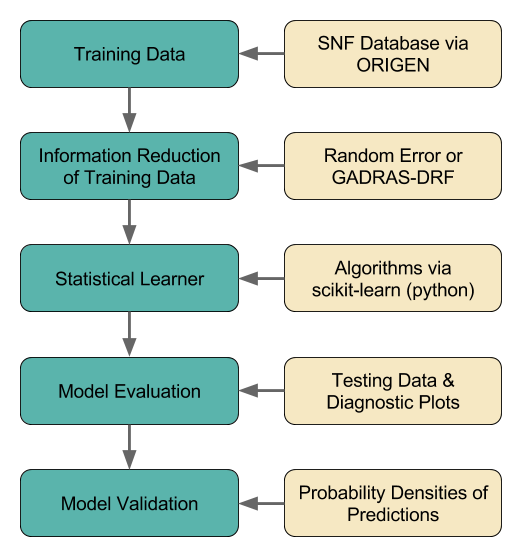
\includegraphics[height=0.85\textheight]{./figures/methodology.png}
  \end{figure}
\end{frame}

\begin{frame}
  \frametitle{Summary}
  \begin{adjustwidth}{-10pt}{0pt}
  \textbf{Pre-detonation nuclear forensics analysis on SNF}\\
  \medskip
  \begin{minipage}{0.35\textwidth}
    \begin{figure}
      \centering
      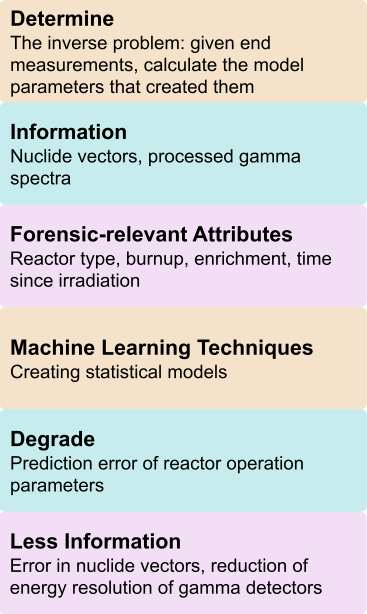
\includegraphics[height=0.75\textheight]{./figures/overview.png}
    \end{figure}
  \end{minipage}%
  \hfill
  \begin{minipage}{0.65\textwidth}
  \begin{itemize}
    \item Demonstrated:
    \begin{itemize}
      \item Simulation of training data set
      \item Information reduction of training set
      \item Prediction of reactor type, burnup, enrichment, and time since irradiation via:
        \begin{itemize}
          \item Maximum Log-Likelihood Calculations
          \item \textit{k}-Nearest Neighbors
          \item Decision Trees
        \end{itemize}
      \item Initial analysis of predictions with respect to information reduction
    \end{itemize}
    \item Simplifications:
    \begin{itemize}
      \item Simulation fidelity (ORIGEN-ARP, homogenized core)
      \item Feature reduction lacks deep inquiry
      \item Simple algorithms, lack of optimization
    \end{itemize}
  \end{itemize}
  \end{minipage}
  \end{adjustwidth}
\end{frame}

\begin{frame}
  \frametitle{Questions \& Next Steps}
  \begin{itemize}
    \item Feature reduction, or lack thereof: show approach?
    \item Improving the comparison/ensuring PHWR representation: redo with same test set for all cases?
    \item Alternatively, can now run 100\% testing for MLL and can use leave-one-out cross validation in scikit
    \item SFCOMPO testing: implement with another method that can handle missing values?
    \item Metrics \& plots: baselines, working on box plots, reactor type accuracy
    \item Energy windows...
  \end{itemize}
\end{frame}

